
\documentclass[a4paper,12pt]{article}
\usepackage[top=1in,bottom=1in,left=1in,right=1in]{geometry}
\usepackage[T1]{fontenc}
\usepackage[utf8]{inputenc}
\usepackage{newunicodechar}
\usepackage{lmodern}
\usepackage{textgreek}
\usepackage{amsmath}
\usepackage{mathtools}
\usepackage{graphicx}
\usepackage{pdflscape}
\usepackage{svg}


\usepackage{tabularx}
\usepackage{blindtext}
\usepackage{hyperref}
\usepackage{pgfgantt}
\usepackage{colortbl}
\usepackage{pdfpages}
\usepackage{setspace}
\usepackage{subcaption}
\usepackage{tikz}
\usepackage{chngcntr}
\usepackage{longtable}
\usepackage{xcolor,colortbl}
\usepackage{pdfpages}

\counterwithin{figure}{subsection}
\usepackage{multicol} 

\setcounter{tocdepth}{3}


\usepackage[backend=bibtex]{biblatex}
\addbibresource{references.bib}


\begin{document}

	\begin{titlepage}
		\newcommand{\HRule}{\rule{\linewidth}{0.5mm}}
		\begin{tikzpicture}[remember picture, overlay]
		\node [anchor=north east, inner sep=0pt]  at (current page.north east)
		{
\includegraphics[width=21cm]{graphics/ucl-banner-dl-port-outline.eps}};
		\end{tikzpicture}\\[3cm]
		\center
		
		\textsc{\Large University College London}\\[0.5cm]
		\textsc{\large Department of Electronic and Electrical Engineering}\\[0.5cm]
		
		\HRule \\[0.4cm]
		\setstretch{1.5}
		{ \huge \bfseries Performance characterisation of 8-bit RISC and OISC architectures}\\[0.4cm]
		\setstretch{1.0}
		\HRule \\[1.0cm]
		
		\begin{multicols}{3}
			
		\Large \emph{Author:}\\
		Mindaugas \textsc{Jarmolovicius}\\
		\href{mailto:zceemja@ucl.ac.uk}{zceemja@ucl.ac.uk}\\
		
		\columnbreak
		
		\Large \emph{Supervisor:}\\
		Prof. Robert \textsc{Killey}\\
		\href{mailto:r.killey@ucl.ac.uk}{r.killey@ucl.ac.uk}
		
		\columnbreak
		
		\Large \emph{Second Assessor:}\\
		Dr. Ed \\\textsc{Romans}\\
		\href{mailto:e.romans@ucl.ac.uk}{e.romans@ucl.ac.uk}
		
		\end{multicols}
		
		\vfill
		\setstretch{2.5}
		{ \large \bfseries A BEng Project Interim Report}\\[1cm]
		\setstretch{1.0}
		{\large December 13, 2019}\\[2cm]
		
	\end{titlepage}

\pagebreak

\begin{multicols}{2}

\section{Abstract}
This is abstract.

\section{Introduction}
Since 80s there been a raise of many processor architectures that try to fulfil specific performance and power application constraints. One of noticeable cases is ARM RISC (Reduced Instruction Set Computer) architecture being used in mobile devices instead of more popular and robust x86 CISC (Complex Instruction Set Computer) architecture in favour of simplicity, cost and lower power consumption \autocite{jamil_1995,blem_menon_sankaralingam_2013}. Its been shown that in low power applications such as IoTs (Internet of Things), OISC\footnote{Also known as URISC (Ultimate Reduced Instruction Set Computer)} (One Instruction Set Computer) implementation can be superior in power and data throughput comparing to traditional RISC architectures \autocite{yokota_saso_hara-azumi_2017, ahmed_sakamoto_anderson_hara-azumi_2015}. This project proposes to compare two novel RISC and OISC architectures and compare their performance, design complexity and efficiency.

Project is split into 3 main objectives:\\
$\bullet$ Design and build a RISC based processor. As it is aimed for low power and performance applications this will be 8bit data size processor with 4 general purpose registers.\\
$\bullet$ Design and build an OISC based processor. There are multiple different implementations such as \texttt{SUBLEQ} or one proposed in chapter \ref{sec:theory}.\\
$\bullet$ Design a fair benchmark that both processors could execute. Benchmark may include different algorithms that are commonly used in controllers, IoT devices or similar low power microprocessor applications.


Following chapters will describe the estimated project outcome, project schedule and work done so far.

\section{The Work Performed to Date}
\subsection{Supporting Theory} \label{sec:theory}
This section explains the theory and predictions of RISC and OISC architectures.

Figure \ref{fig:simple_blocks} represents simplified diagrams of RISC and OISC architectures. In RISC architecture, program data travels from program memory to control block where instruction is decoded and further decided where what data is directed. Such structure requires complicated control block and additional data routing blocks. In order to increase performance of such processor one would need to add pipelining or add multiple cores. Both methods bring big disadvantages - multicore processor requires software adjustments and each core doubles the control and datapath substantially increasing die area; pipelinig allow operation at higher frequencies however it brings design complications such as complicated hazard prevention logic and instruction lookup. Simplicity of OISC architecture overcomes these disadvantages by following:
Pipelining can be done by individual blocks and programmibly waiting for results, multicore can be simulated by adding more data and instruction buses, hazards can be prevented with software or/and integrated into address registers. 
Furthermore, ALU and any other processor component can be divided by adding different address registers thus allowing to utilise multiple components at the same time given that multiple data buses are used. 

\begin{figure*}[h!]
	\centering
	\begin{subfigure}[b]{1\textwidth}
		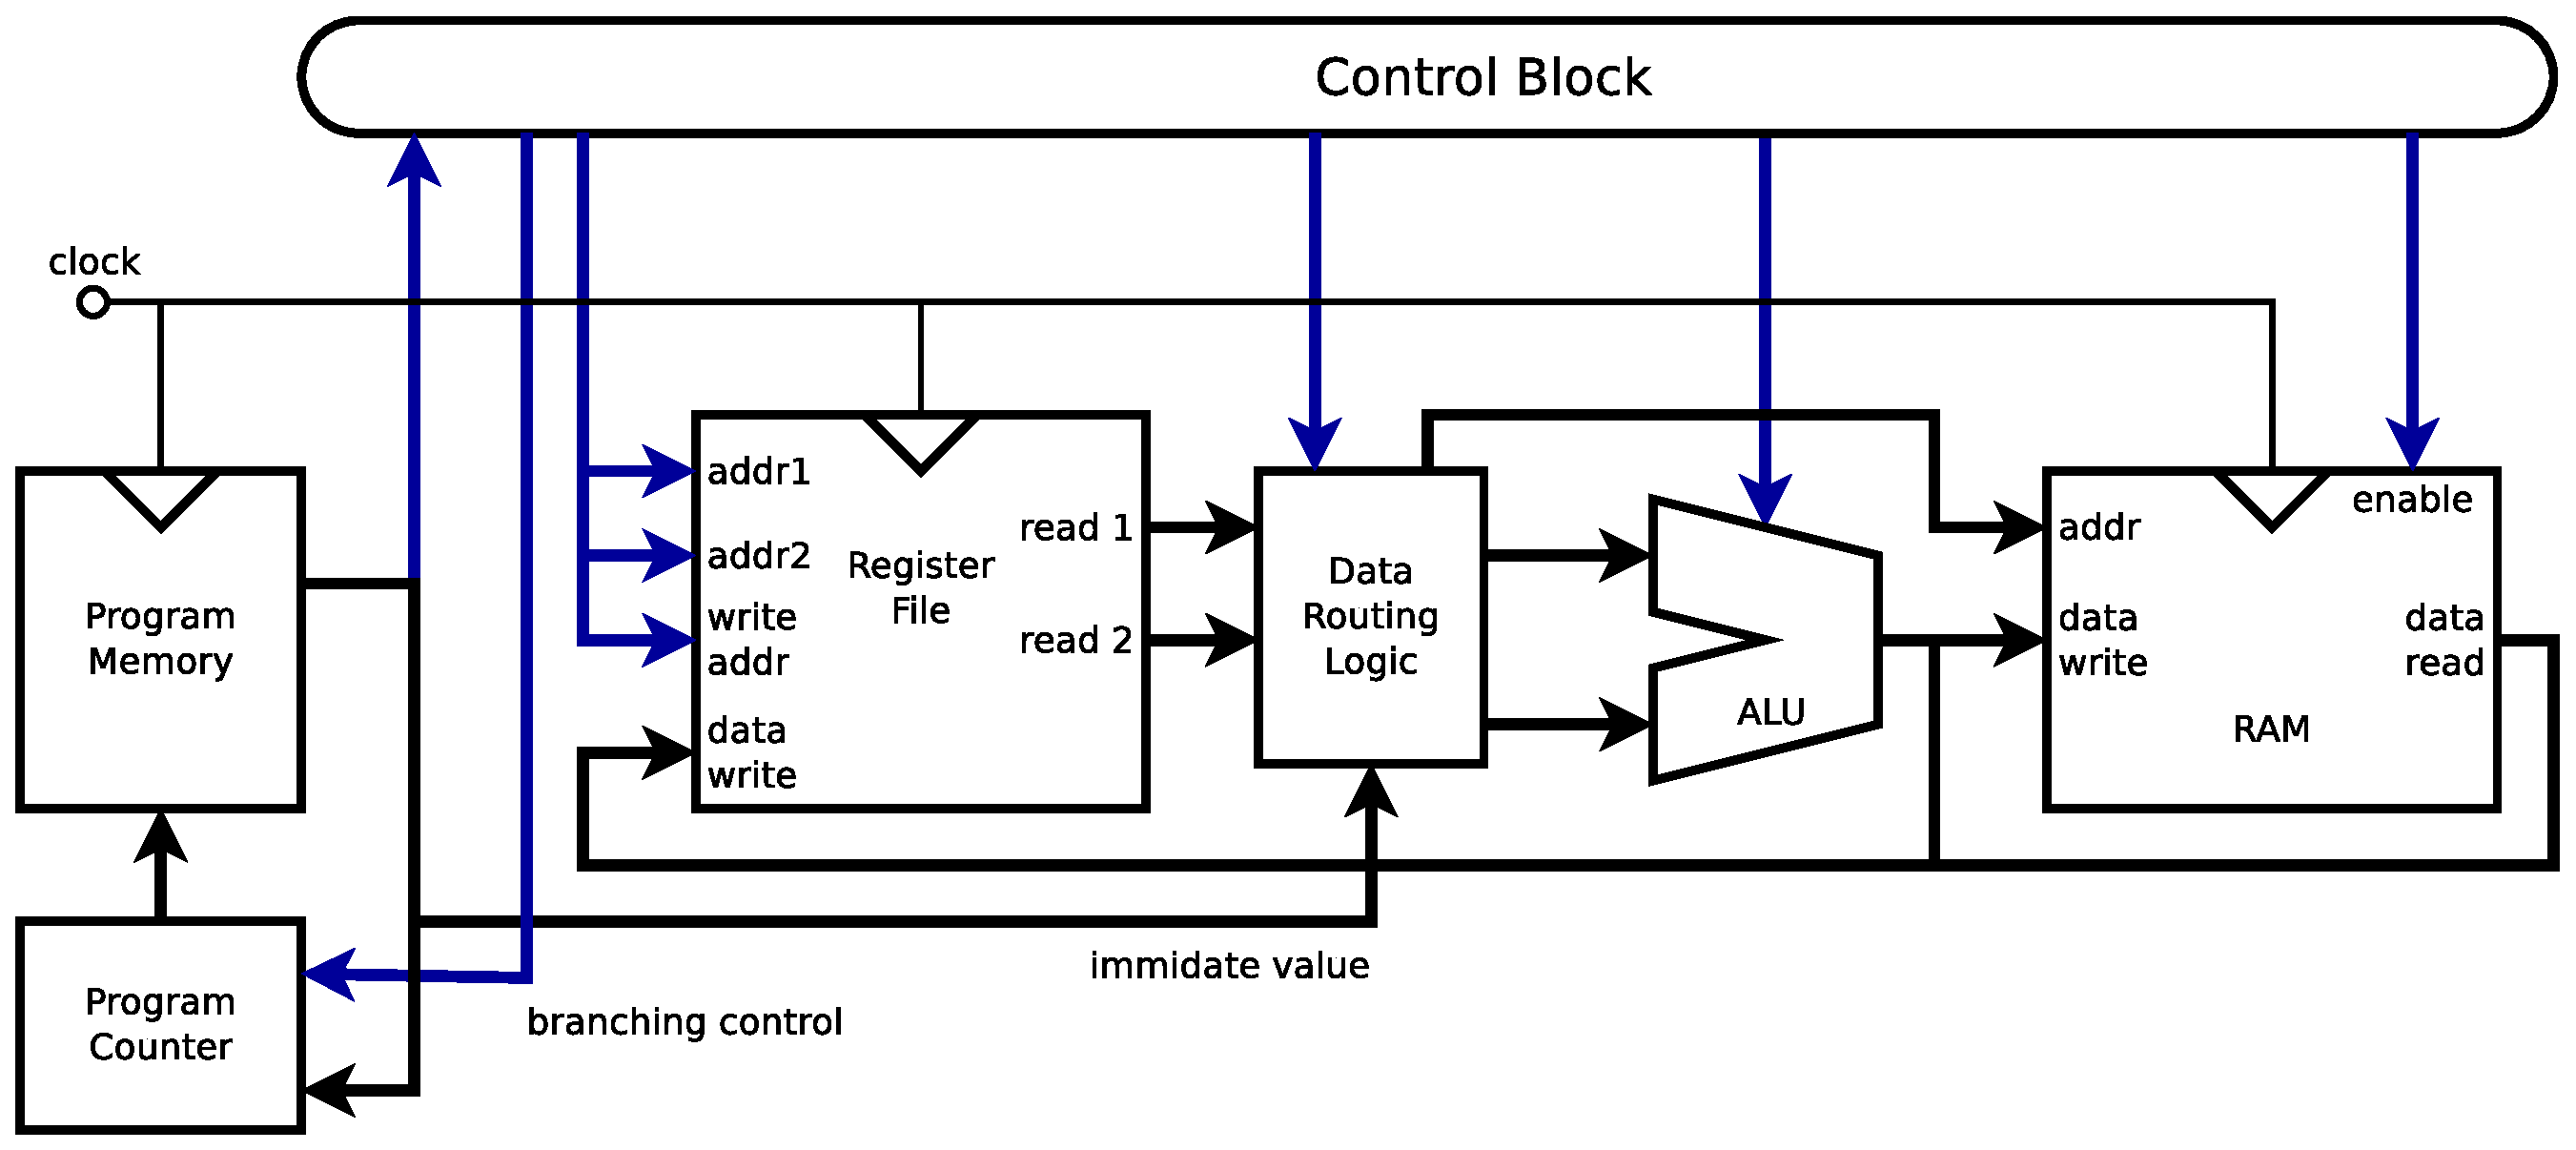
\includegraphics[width=\linewidth]{graphics/risc.eps}
		\caption{RISC microarchitecture diagram}
		\label{fig:risc_simple}
	\end{subfigure}
	
	\begin{subfigure}[b]{1\textwidth}
		\includegraphics[width=\linewidth]{graphics/oisc.eps}
		\caption{Single data bus OISC microarchitecture diagram}
		\label{fig:oisc_simple}
	\end{subfigure}
	
	\caption{Simplified diagrams of both architectures. Blue lines indicate control/instruction buses and black - data buses}
	\label{fig:simple_blocks}
\end{figure*}

\end{multicols}
\newpage
\begin{landscape}
	\subsection{Project Scheduling}
	As it can be seen in table \ref{table:time} below, project is mainly split into Term 1 which is dedicated for RISC and Term 2 which is dedicated for OISC implementation. Approximately 3 weeks are left until final report to have enough spare time to finish all tests and complete poster \& report itself. It is also expected to have a lot of coursework around this time.
	\begin{table}[h!]
		\centering
		\begin{ganttchart}[
			y unit title=0.4cm,
			y unit chart=0.5cm,
			x unit=1.1mm,
			hgrid,
			today=2019-12-13,
			today label node/.append style={below=12pt},
			today label font=\itshape\color{blue},
			today rule/.style={draw=blue, ultra thick},
			title height=1,
			bar/.append style={fill=blue!50},
			bar incomplete/.append style={fill=gray!50},
			progress label text={$\displaystyle{#1\%}$},
			time slot format=isodate
			]{2019-10-01}{2020-03-31}
			\gantttitlecalendar{year, month=shortname} \\
			\gantttitle{40}{6}
			\gantttitlelist{41,...,52}{7}
			\gantttitlelist{1,...,13}{7}
			\gantttitle{}{2} \\
			\ganttbar[progress=100]{RISC implementation}{2019-10-01}{2019-10-27}\\
			\ganttbar[progress=90]{RISC Optimisations}{2019-10-27}{2019-11-25}\\
			\ganttbar[progress=100]{UART and I/O}{2019-10-21}{2019-10-27}
			\ganttbar[progress=100]{}{2019-11-25}{2019-12-08} \\
			\ganttbar[progress=100]{RISC Assembler}{2019-10-14}{2019-11-11}\\
			\ganttbar[progress=20]{Developing benchmark}{2019-11-11}{2019-12-13}
			\ganttbar[progress=0]{}{2020-02-23}{2020-03-07} \\
			\ganttbar[progress=10]{OISC Implementation}{2019-12-02}{2019-12-13}
			\ganttbar[progress=0]{}{2020-01-13}{2020-02-02}\\
			\ganttbar[progress=0]{OISC Optimisations}{2020-02-02}{2020-02-23}\\
			\ganttbar[progress=0]{OISC Assembler}{2020-01-20}{2020-02-09}\\
			\ganttbar[progress=0]{OISC Compiler}{2020-02-09}{2020-03-01}\\
			\ganttmilestone{Project Proposal finalised}{2019-10-14}\\
			\ganttmilestone{Progress Report \#1}{2019-11-04}\\
			\ganttmilestone{Progress Report \#2}{2019-11-25}\\
			\ganttmilestone{December Interim Report}{2019-12-13}\\
			\ganttmilestone{Progress Report \#3}{2020-01-20}\\
			\ganttmilestone{Progress Report \#4}{2020-02-14}\\
			\ganttmilestone{Progress Report \#5}{2020-03-02}\\
			\ganttmilestone{Poster Presentation}{2020-03-18}\\
			\ganttmilestone{Final Report}{2020-03-30}\\
			\ganttvrule{Reading Week}{2019-11-03}
			\ganttvrule{}{2019-11-10}
			\ganttvrule[vrule label node/.append style={anchor=north west}]{Holidays}{2019-12-13}
			\ganttvrule{}{2020-01-12}
			\ganttvrule{Reading Week}{2020-02-17}
			\ganttvrule{}{2020-02-23}
		\end{ganttchart}	
		\caption{Project schedule Grantt chart}
		\label{table:time}
	\end{table}
\end{landscape}
\pagebreak

\begin{multicols}{2}

\subsection{Progress to Date}
Use as many sections as you need to in order to discuss your progress so far. For example, you can use a different section to discuss each bit of the system to be constructed or designed.Include difficulties and issues impeding progress.


\subsubsection{Memory}
Initial plan was to use 32M-Word 16bit SDRAM chip located at FPGA board. After successfully simulating most of processor functions, next step was to synthesise and run it on FPGA which brought 2 problems: (1) Uploading program into ROM is not simple as generic Verilog unpacked register array cannot be initialised from file. Solution to this problem was solved by using FPGA built-in M9K memory that allows flexible RAM/ROM configuration. In addition, M9K memory can be read from/written to via JTAG connection without affecting FPGA operation which enabled quick method to upload programs without need to resynthesising processor code.

(2) Timing of SDRAM memory controller runs at much higher frequency than processor (at 100MHz versus 1MHz), initial implementation of interface between them was multiple 1-word length FIFO registers which caused memory read operation take 2 processor cycles. 3 possible solutions were considered - suspend processor clock while memory data is read which would harm performance; remove FIFO registers and rely on SDRAM clock being much greater than processor clock which is not ideal if higher processor clocks are intended to be used; use M9K. Last option was chosen due to ease of implementation and ability to read RAM content via JTAG for debugging purposes.

\end{multicols}
\newpage
\subsubsection{Instructions}
Table \ref{table:risc_instr} below represents RISC processor instructions that been implemented so far.
\arrayrulecolor{black}
\begin{longtable}{| l | p{.70\textwidth} | c |}
	\hline 
	\rowcolor[rgb]{0.82,0.82,0.82}
	Instr. & Description & Completed \\\hline
		

	\multicolumn{3}{|c|}{
		\cellcolor[rgb]{0.7,0.7,1}\textit{2 register instructions}} \\\hline
	\arrayrulecolor[rgb]{0.82,0.82,0.82}
		
	MOVE & Copy intimidate or register & x \\\hline
	ADD  & Arithmetical addition & x \\
	SUB  & Arithmetical subtraction & x \\
	AND  & Logical AND & x \\
	OR   & Logical OR & x \\
	XOR  & Logical XOR & x \\
	MUL  & Arithmetical multiplication & x \\
	DIV  & Arithmetical division (inc. modulus) & x \\
		

	\arrayrulecolor{black}\hline
	\multicolumn{3}{|c|}{
		\cellcolor[rgb]{0.7,0.7,1}\textit{1 register instructions}} \\
	\hline\arrayrulecolor[rgb]{0.82,0.82,0.82}
	
	CI0  & Replace intimidate value byte 0 for next instruction & x \\
	CI1  & Replace intimidate value byte 1 for next instruction & x \\
	CI2  & Replace intimidate value byte 2 for next instruction & x \\\hline
		
	SLL  & Shift left logical & \\
	SRL  & Shift right logical & \\
	SRA  & Shift right arithmetical & \\\hline
		
	LWHI & Load word (high byte) & x \\
	SWHI & Store word (high byte, reg. only) & x \\
	LWLO & Load word (low byte) & x \\
	SWLO & Store word (low byte, stores high byte reg.) & x \\\hline
		
	INC  & Increase by 1 & x \\
	DEC  & Decrease by 1  & x \\
	GETAH& Get ALU high byte reg. (only for MUL \& DIV) & x \\
	GETIF& Get interrupt flags & x \\\hline
		
	PUSH & Push to stack & x \\
	POP  & Pop from stack & x \\
	COM  & Send/Receive to/from com. block & x \\\hline
	
	ADDI & Arithmetical addition with intimidate & x \\
	SUBI & Arithmetical subtraction with intimidate & x \\
	ANDI & Logical AND with intimidate & x \\
	ORI  & Logical OR with intimidate & x \\
	XORI & Logical XOR with intimidate & x \\\hline
	
	BEQ  & Branch on equal & x \\
	BGT  & Branch on greater than & x \\
	BGE  & Branch on greater equal than & x \\
	BZ   & Branch on zero & x \\
		
	\arrayrulecolor{black}\hline
	\multicolumn{3}{|c|}{
		\cellcolor[rgb]{0.7,0.7,1}\textit{0 register instructions}
	} \\
	\hline\arrayrulecolor[rgb]{0.82,0.82,0.82} 
		
	CALL & Call function, put return to stack & x \\
	RET  & Return from function & x \\
	JUMP & Jump to address & x \\
	RJUMP& Relative jump & \\\hline
	RETI & Return from interrupt & x \\
	INTRE& Set interrupt entry pointer & x \\\hline
	
	CLC  & Clear ALU carry-in & \\
	SETC & Set ALU carry-in & \\
	CLS  & Clear ALU sign & \\
	SETS & Set ALU sign & \\
	SSETS& Enable ALU sign & \\
	CLN  & Clear ALU negative & \\
	SETN & Set ALU negative & \\
	SSETN& Enable ALU negative & \\

		
	\arrayrulecolor{black}\hline
	
	\caption{Instruction set for RISC processor}
	\label{table:risc_instr}
\end{longtable}	


\subsubsection{Program Counter}
\begin{figure*}[h!]
	\centering
	%\def\svgwidth{16cm}
	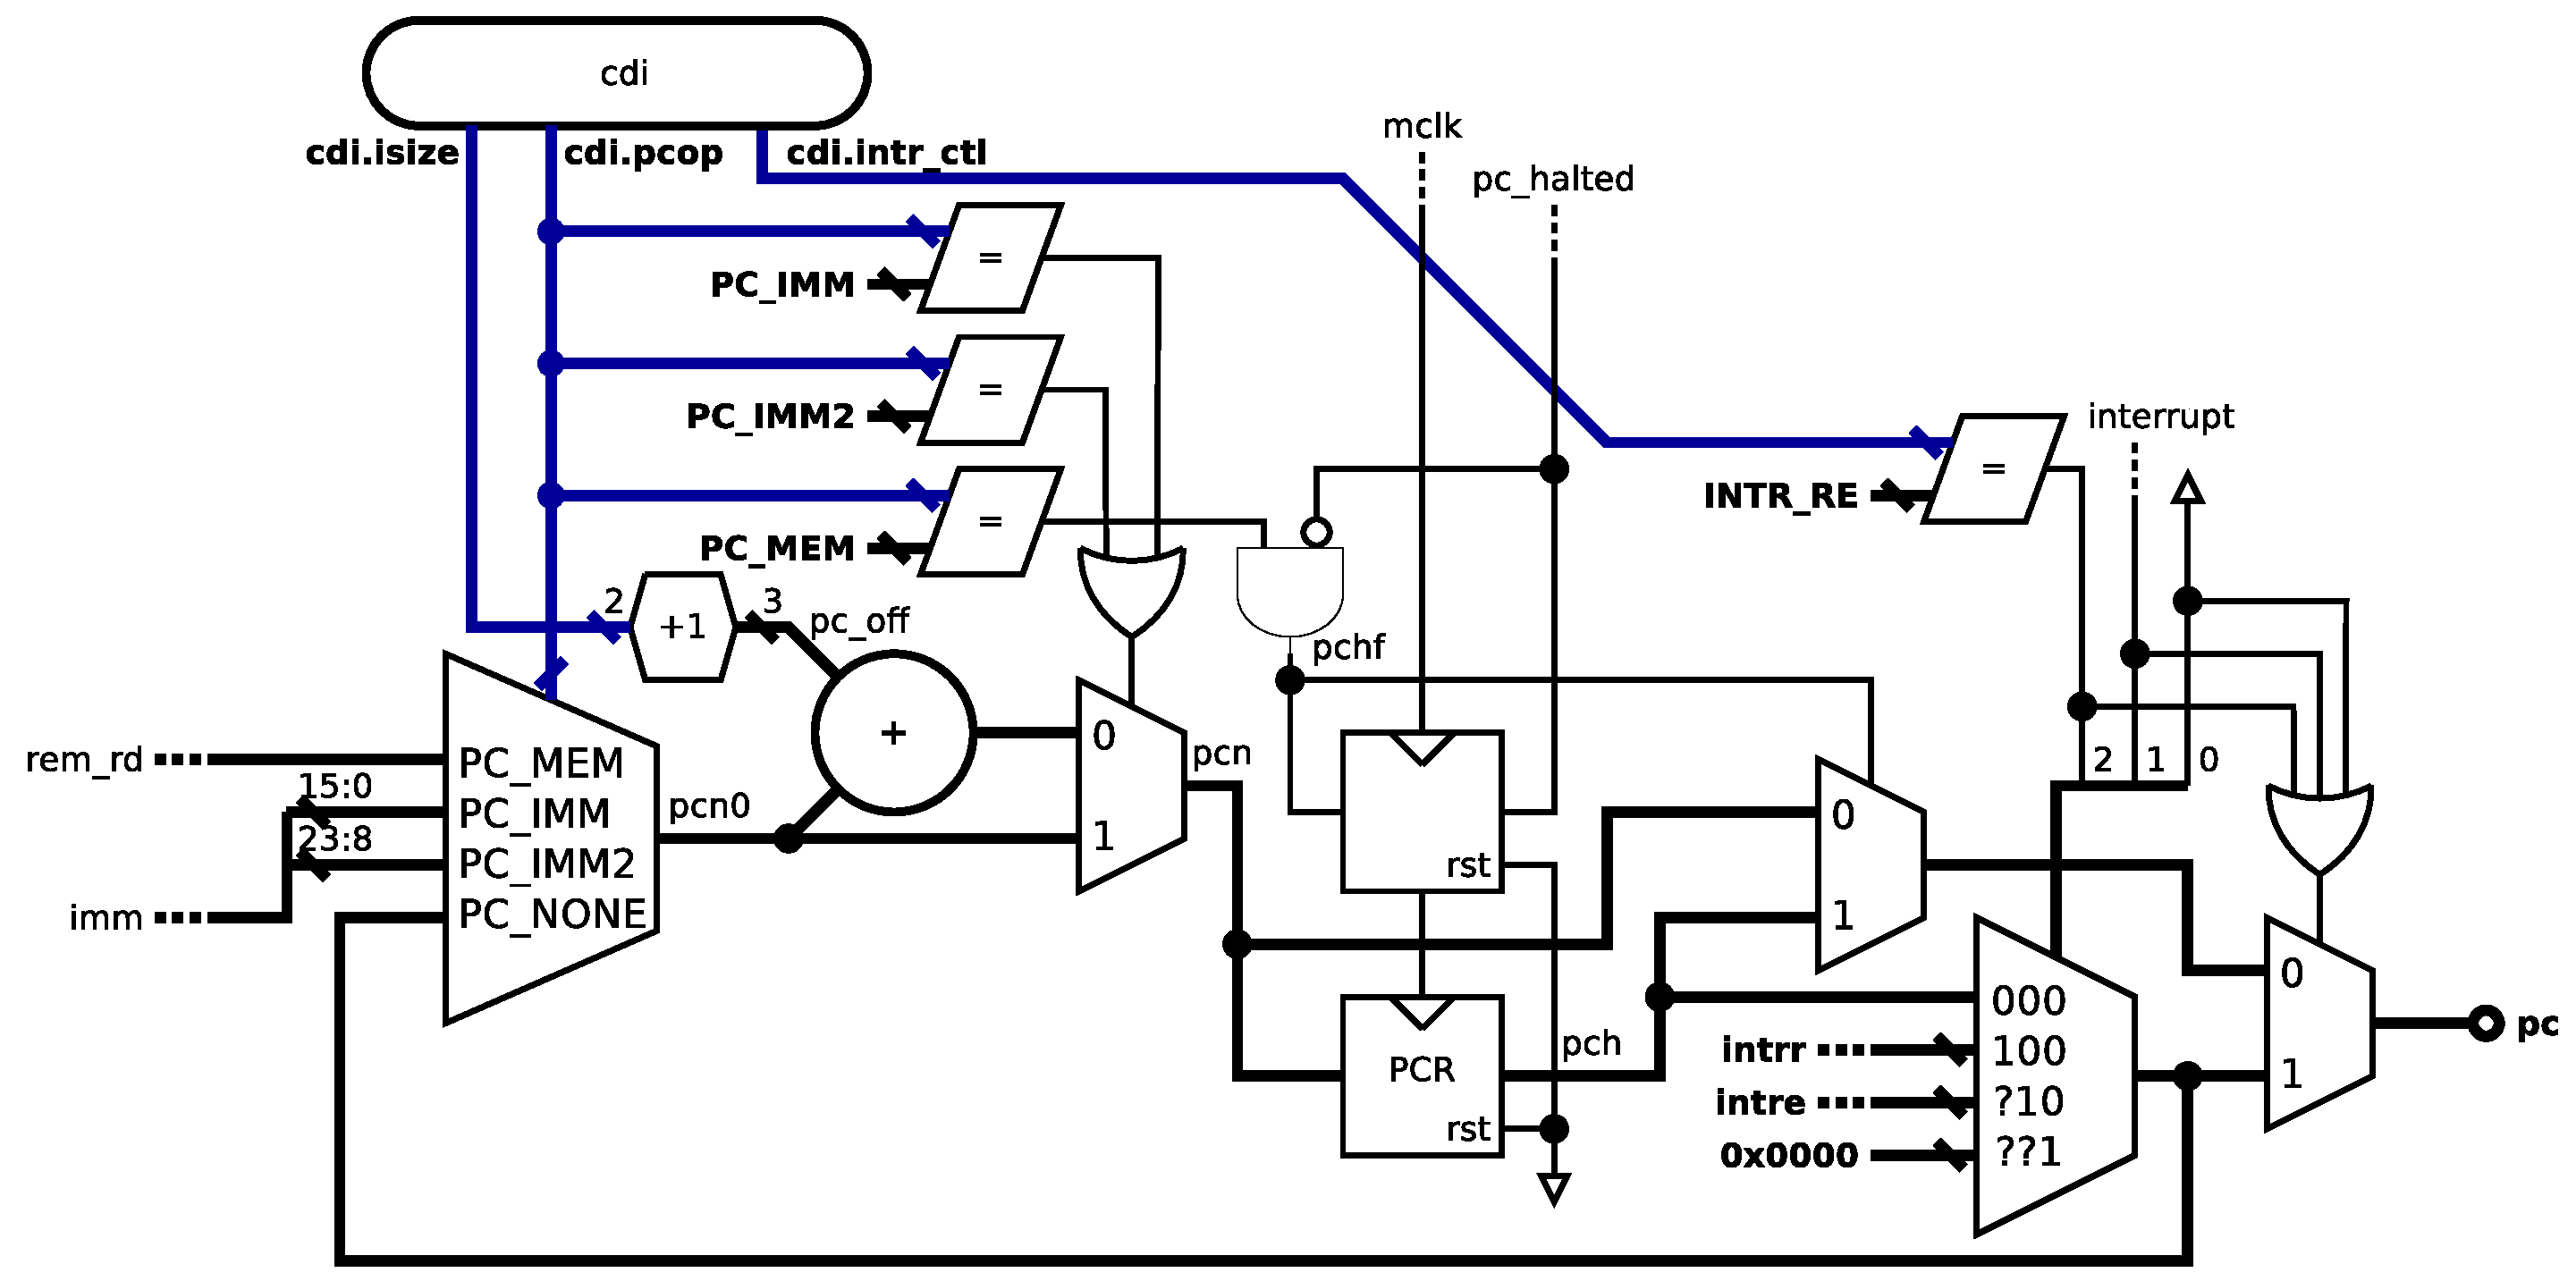
\includegraphics[width=\linewidth]{graphics/program_counter.eps}
	\caption{Digital diagram of RISC8 program counter}
	\label{fig:program_counter}
\end{figure*}


\subsubsection{Stack Pointer}
\begin{figure*}
	\centering
	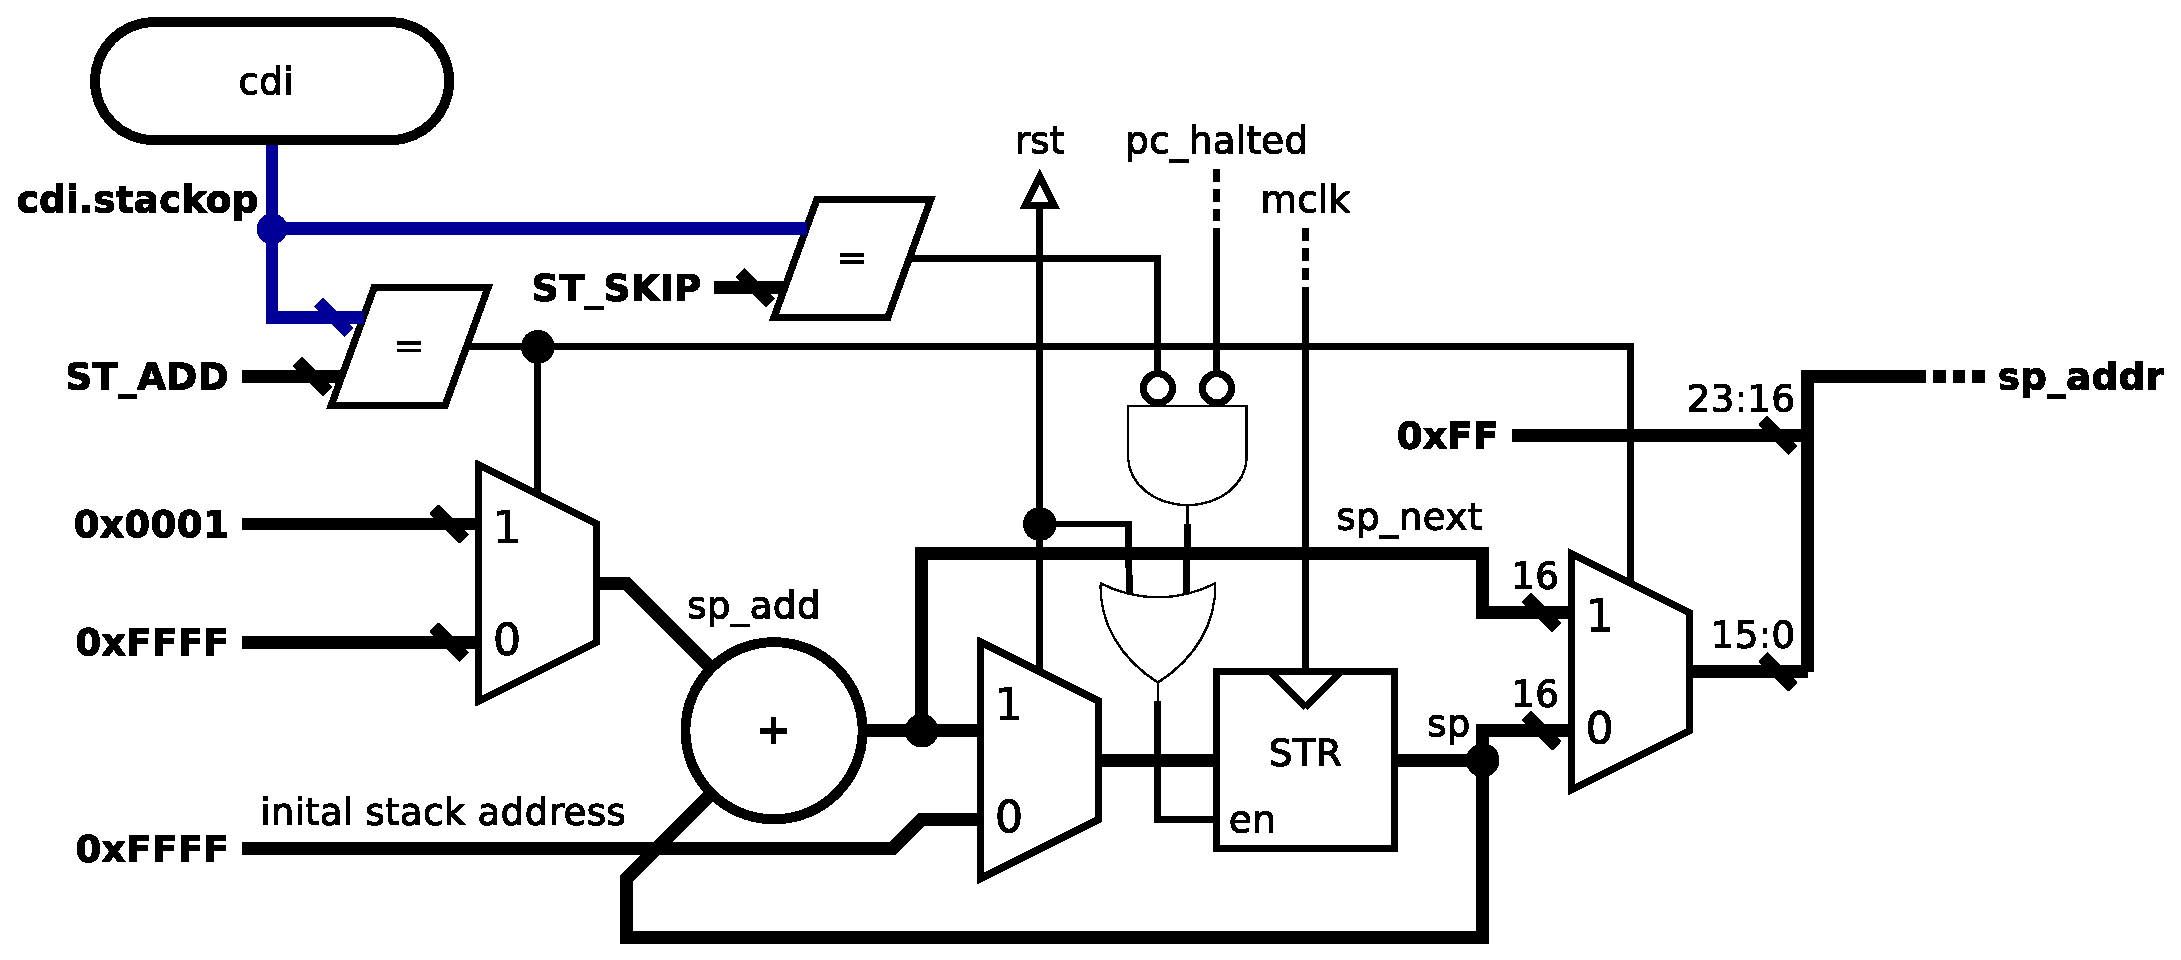
\includegraphics[width=\linewidth]{graphics/stack_diagram.eps}
	\caption{Digital diagram of RISC8 program counter}
	\label{fig:stack_pointer}
\end{figure*}


\section{Summary of Difficulties and Issues}
\begin{multicols}{2}
This chapter focuses on any difficulties and issues that are hindering project from moving forward.

\subsection{List of Difficulties}

List of difficulties currently encounter:
\begin{description}
	\item[$\bullet$] Benchmark
	\item[$\bullet$] Assembler/Compiler
\end{description}

\subsubsection{Benchmark}
One of the difficulties is to design an appropriate benchmark that could test scenarios used in actual such processor applications. Other issue comes with writing benchmark itself, for instance benchmark test to finding prime number may have used many different algorithms where one of the fastest and used in actual industry may be "Sieve of Atkin" algorithm \autocite{morain_1989}, however is it fairly complicated and time consuming especially when written in assembly. 

\subsubsection{Assembler/Compiler}
In order to write more complicated code for benchmark, a proper compiler is required. Current assembler support definitions and labels, however not macros or imports from other files, nor linked libraries. Ideally, a common language compiler needs to be developed so that benchmark programs could be imported without need to completely rewrite them in assembly. However such compiler might take more time to develop than writing benchmarks in assembly. Therefore it needs to be decided which option to do.

\subsection{Failure Assessment}
This section describes likely possibilities of project failures:

As of current schedule OISC processor will be implemented in Term 2, however due to personal schedule project will be given about twice less time than in Term 1 which may result in not finishing OISC processor or developing all benchmarks for it on time. Mitigation for this is to closely follow schedule and adjust OISC design in such way as it would take less time to implement benchmark.

Another possibility may be FPGA failure which would delay testing and benchmarking processors.

\subsection{Updated Safety Risk Assessment}
There are no changes to Safety Risk Assessment.

\end{multicols}

\section{Appendix A: Safety Risk Assessment}
RiskNet report is appended at the end of this document.

\section{Appendix B: Computer Code}
Append any code you may need here. Reference it in the text as "Appendix B, code snippet \#"; for example,"Finda sample of the code usedfor this experiment in Appendix B, code snippet 2".

\section{References}
\printbibliography

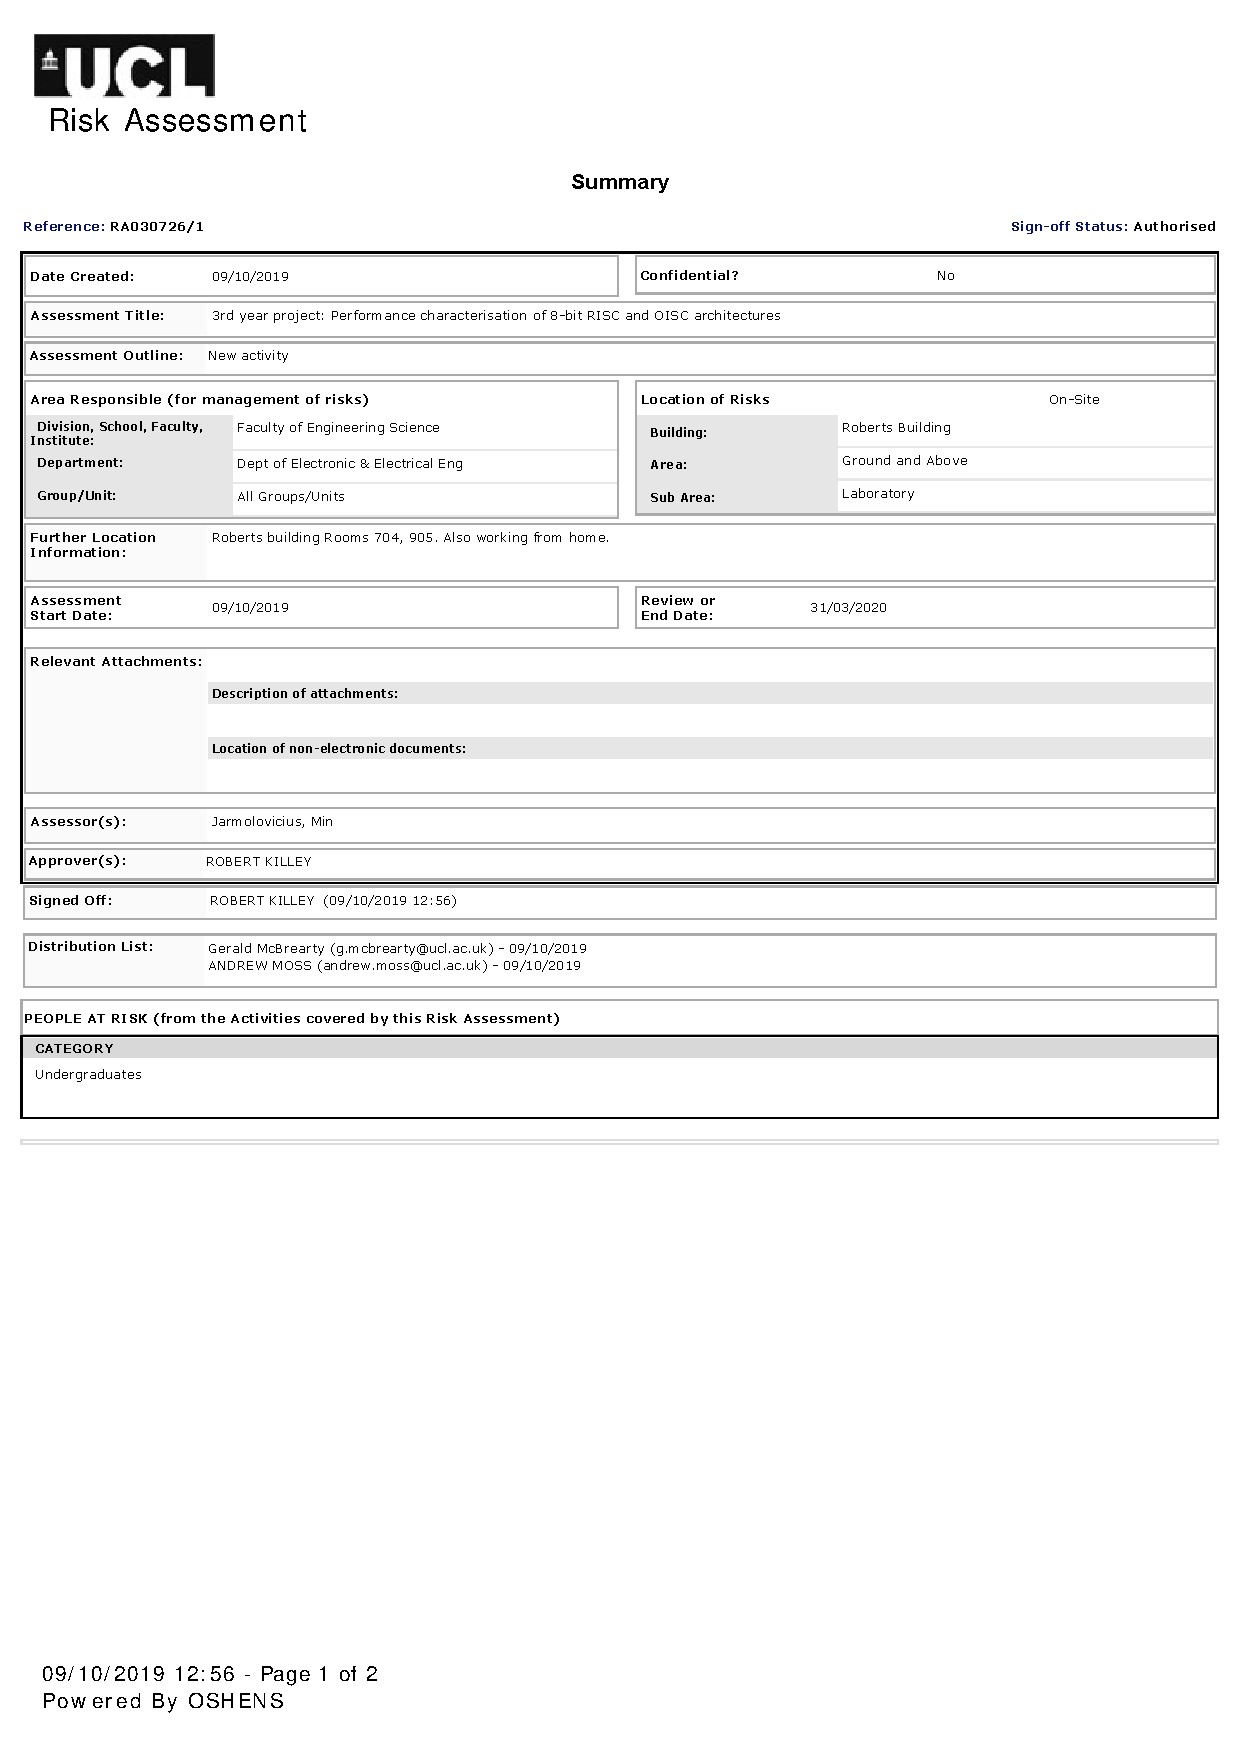
\includepdf[pages=-]{risknet.pdf}

\end{document}